% Possible aspect ratios are: 169, 1610, 149, 54, 43 and 32.
\documentclass[aspectratio=1610,9pt]{beamer} % test beamer document
\usepackage[T1]{fontenc}
\usepackage[cache=false]{minted}
\renewcommand{\MintedPygmentize}{pygmentize-3.4}
\usepackage{wrapfig}
\usetheme{ncas}
\definecolor{lightyellow}{HTML}{FFFFE0}
\title{Data Acquisition from Serial Ports}

\subtitle{With Python's pyserial module}

\author{Dan Walker}

\begin{document}

\begin{frame}
\titlepage
\end{frame}

\begin{frame}
\frametitle{Serial Ports}

\section{What is a serial port?}

\begin{quote}
In computing, a serial port is a serial communication physical interface
through which information transfers in or out one bit at a time (in
contrast to a parallel port). Throughout most of the history of personal
computers, data was transferred through serial ports to devices such as
modems, terminals and various peripherals.
\end{quote}

(ref: \href{http://en.wikipedia.org/wiki/Serial_Port}{Wikipedia} )

\begin{itemize}
\itemsep1pt\parskip0pt\parsep0pt
\item
  Very basic form of communication. Low power, low CPU.
\item
  Protocol is called ``RS-232'' or ``RS-485''
\item
  In common use on scientific equipment, for example NCAS's laser
  ceilometer.
\item
  Usually a 9-pin or 25-pin ``D-Sub'' port, but sometimes a variety of
  others
\item
  no longer common on computers. However, USB-\textgreater{}Serial
  adapters are approx £15.
\end{itemize}

\end{frame}
\begin{frame}
\frametitle{The Papouch temperature probe}

\begin{wrapfigure}[4]{r}{0.45\textwidth}
\vspace{-3cm}
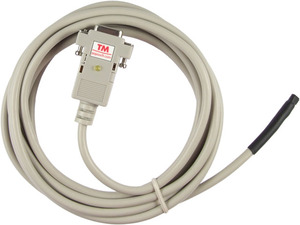
\includegraphics[width=0.45\textwidth]{papouchprobe.jpeg}
\end{wrapfigure}
\par
\begin{minipage}{0.45\textwidth}
\begin{itemize}
\itemsep1pt\parskip0pt\parsep0pt
\item
  Very basic serial RS232 temp probe
\item
  approx €20
\item
  Measures temperatures from -55°C to +125°C, 0.1°C resolution
\item
  Output is in ASCII format in °C, no conversion needed.
\item
  Port powered so needs no power source
\item
  Datasheet included in your kit
\end{itemize}
\end{minipage}

\end{frame}
\begin{frame}[fragile=singleslide]
\frametitle{Basic connections}

\href{https://pythonhosted.org/pyserial/shortintro.html}{https://pythonhosted.org/pyserial/shortintro.html}

\begin{minted}[bgcolor=lightyellow]{python}
#!/usr/bin/env python
import serial

ser = serial.Serial(
   port='/dev/ttyUSB0',
   baudrate=9600,
   bytesize=serial.EIGHTBITS,
   parity=serial.PARITY_NONE,
   stopbits=serial.STOPBITS_ONE
)
\end{minted}

\subsection{Exercise}

Figure out how to read and return data from the \texttt{ser} object.

As well as the pyserial shortintro above, you may find
\url{https://pythonhosted.org/pyserial/pyserial_api.html}
and the Papouch thermometer datasheet useful.

\subsubsection{Q1. Why doesn't \texttt{readline()} work (easily)?}

\end{frame}
\begin{frame}[fragile]
\frametitle{Basic connections example}

\begin{itemize}[<+->]
\itemsep1pt\parskip0pt\parsep0pt
\item<1->
  baudrate, bytesize, parity and stopbits are the most common parameters
  that need changing
\item<2->
  They depend on the serial device in question
\item<3->
  The Papouch thermometer 9600 baud, eight bits, no parity checking and
  one stopbit. (``9600 8N1'') (Same as pyserial's defaults!)
\item<4->
  For other parameters, see pyserial's API (
  \href{https://pythonhosted.org/pyserial/pyserial_api.html}{https://pythonhosted.org/pyserial/pyserial\_api.html}
  )
\end{itemize}
\end{frame}
\begin{frame}[fragile]

\begin{minted}[bgcolor=lightyellow]{python}
#!/usr/bin/env python

import serial

ser = serial.Serial(
   port='/dev/ttyUSB0',
)

print(ser.read(size=8)) # "8" here is specific to the Papouch thermometer device

ser.close()
\end{minted}

\begin{verbatim}
$ python readserial_basic.py
b'+018.9C\r'
\end{verbatim}

\end{frame}
\begin{frame}[fragile]
\frametitle{Basic connections example - 2}

\subsubsection{A note on port names}

\begin{itemize}
\itemsep1pt\parskip0pt\parsep0pt
\item
  \texttt{/dev/ttyUSB0} is Linux's way of referring to the first USB
  serial port
\item
  subsequent ones \texttt{/dev/ttyUSB1}, \texttt{/dev/ttyUSB2} and so-on
\item
  Built-in serial ports would be \texttt{/dev/ttyS0},
  \texttt{/dev/ttyS1} etc.
\item
  Windows machines, the portname will be of the form \texttt{COM1},
  \texttt{COM2}, \texttt{COM3}, etc. (USB ports \emph{normally} start at
  \texttt{COM3}, but not always)
\item
  Mac OSX machines are different again. It will be something like
  \texttt{/dev/tty.SOMETHING}, e.g. \texttt{/dev/tty.PL2303-xxx}
\item
  You may need to experiment to determine which the USB converter has
  attached to.
\item
  More on this later
\end{itemize}

\end{frame}
\begin{frame}[fragile]
\frametitle{Why \texttt{ser.read(size=8)} ?}
If you refer to the
\href{http://www.papouch.com/en/shop/product/tm-rs232-thermometer/tm_en.pdf}{Papouch
thermometer datasheet} 's ``Communication Protocol'' section, you will
see:

\begin{verbatim}
<sign><3 characters – integer °C>
<decimal point><1 character – tenths of °C>
<C><Enter>
\end{verbatim}

as a description of the output. In ASCII coding, each character is one
byte so each temperature from the thermometer is eight bytes.

\end{frame}
\begin{frame}
\frametitle{The \texttt{datetime} module}

For the data to be useful you need to add a date and time reading.
Python includes a standard module for this, \texttt{datetime} (
\url{https://docs.python.org/3/library/datetime.html}
)
\begin{itemize}
\item Can process times in a very wide variety of formats
\item Can deal with different timezones (if you ask it to)
\item Other date/time modules are available, but \texttt{datetime} is alwyas avaiable.
\end{itemize}
\end{frame}
\begin{frame}[fragile]
\frametitle{Date and Time formats}

\begin{itemize}
\itemsep1pt\parskip0pt\parsep0pt
\item
  Timezone should be in UTC or TAI in the majority of cases
\item
  Use an unambiguous format
\item
  \texttt{isoformat()} produces a standard format by default - rarely is
  that a problem.
\item
  \texttt{strftime()} will do any format you require (e.g. for documents
  intended to be read by people)
\end{itemize}


\subsection{Exercise}

Add date and time to your output.

\subsubsection{Q1. What time format should you use?
Why?}

\subsubsection{Q2. Which timezone?}

\subsubsection{Q3. Are you sure the datetime call and the reading are at
the same time? (within
reason)}

\end{frame}
\begin{frame}[fragile]
\frametitle{Time and Date example}

\begin{minted}[bgcolor=lightyellow]{python}
#!/usr/bin/env python

from datetime import datetime
import serial

ser = serial.Serial(
   port='/dev/ttyUSB0',
   baudrate=9600,
)

print(datetime.utcnow().isoformat(), ser.read(size=8))

ser.close()
\end{minted}
\end{frame}
\begin{frame}[fragile]

\texttt{datetime.utcnow().isoformat()} is, as you might expect, a
command to return the current UTC in ISO format, e.g.:

\texttt{2018-09-28T13:24:39.773878 b'+018.8C\r'}

\begin{verbatim}
print(datetime.utcnow().isoformat(), ser.read(size=8))
\end{verbatim}

\begin{itemize}
\itemsep1pt\parskip0pt\parsep0pt
\item
  \texttt{datetime.utcnow()} call can return in advance of the
  \texttt{ser.read()} call (run \texttt{readserial\_example\_advance\_read.py} to demonstrate this) 
\item
  timestamp and the temperature should be as close as possible
\item
  store the data in a variable and output the variable and the time at
  the same time
\end{itemize}

\begin{verbatim}
datastring = ser.read(size=8)
print(datetime.utcnow().isoformat(), datastring)
\end{verbatim}

\end{frame}
\begin{frame}[fragile]
\begin{verbatim}
Python 3.6.5 |Anaconda, Inc.| (default, Apr 29 2018, 16:14:56)
[GCC 7.2.0] on linux
Type "help", "copyright", "credits" or "license" for more information.
>>> from datetime import datetime
>>> dt = datetime.now()
>>> print(dt)
2018-09-28 14:27:40.039017
>>> dt
datetime.datetime(2018, 9, 28, 14, 27, 40, 39017)
>>> print(dt.strftime('%Y-%m-%d %H:%M:%S'))
2018-09-28 14:27:40
>>> print(dt.strftime('%A, %B %d, %Y'))
Friday, September 28, 2018
\end{verbatim}

\end{frame}
\begin{frame}
\frametitle{Continuous logging}

You are probably going to want your data capture code to run
indefinitely, or at least more than once. You should be familiar with
flow control and looping constructs from your Intro To Python.

\subsection{Exercise}

Add a loop to your code to continuously log the reading and time.

\subsubsection{Q1. What sort of looping construct are you using?
Why?}

\subsubsection{Q2. What condition causes the loop to
exit?}

\subsubsection{Further exercise if you have
time.}

Try and get the same output using \texttt{readline()} instead. Why might
this be preferable for other instruments?

\end{frame}
\begin{frame}[fragile]
\frametitle{Continuous logging example}

In most cases, you will need to log more than one data point. A basic
modification is fairly simple, using a \texttt{while} loop:

\begin{minted}[bgcolor=lightyellow]{python}
#!/usr/bin/env python

from datetime import datetime
import serial

ser = serial.Serial(
   port='/dev/ttyUSB0',
   baudrate=9600,
)

while ser.isOpen():
   datastring = ser.read(size=8)
   print(datetime.utcnow().isoformat(), datastring)

ser.close()
\end{minted}

returns something like:

\begin{verbatim}
2018-09-28T13:30:56.788659 b'+018.8C\r'
2018-09-28T13:31:06.780694 b'+018.7C\r'
2018-09-28T13:31:16.770664 b'+018.8C\r'
2018-09-28T13:31:26.762724 b'+018.7C\r'
\end{verbatim}

\end{frame}
\begin{frame}[fragile]
\frametitle{Continuous logging with \texttt{readline()}}

\begin{itemize}
\itemsep1pt\parskip0pt\parsep0pt
\item
  The example thermometer \emph{always} returns exactly eight bytes, and
  so \texttt{ser.read(size=8)} is fine.
\item
  instruments do not always return fixed-length data, and instead
  separate the readings (or sets of readings) with a special character.
\item
  Usually \href{http://en.wikipedia.org/wiki/Newline}{newline} or
  \href{http://en.wikipedia.org/wiki/Carriage_return}{carriage return}
\item
  The pyserial module provides \texttt{readline()} to handle this case.
\item
  worked differently prior to python v2.6
\end{itemize}
\end{frame}
\begin{frame}[fragile]

\begin{minted}[bgcolor=lightyellow]{python}
#!/usr/bin/env python

from datetime import datetime
import serial
import io

ser = serial.Serial(
   port='/dev/ttyUSB0',
   baudrate=9600,
)

sio = io.TextIOWrapper(io.BufferedRWPair(ser, ser, 1), encoding='ascii', newline='\r')
#Needed for Python 3
sio._CHUNK_SIZE =1

while ser.isOpen():
   datastring = sio.readline()
   print(datetime.utcnow().isoformat(), datastring)

ser.close()
\end{minted}

\end{frame}
\begin{frame}
\frametitle{Outputting to a file}

Usually you will want to output the data to a file rather than the
terminal, so, e.g., the data are on disk in case of a fault or similar.

\subsection{Exercise}

Alter your code to write the data out to a file.

\end{frame}
\begin{frame}[fragile]
\frametitle{Outputting to a file
example}

\begin{minted}[bgcolor=lightyellow]{python}
#!/usr/bin/env python
'''This version of the readserial program demonstrates
using python to write an output file'''

from datetime import datetime
import serial, io

outfile='/tmp/serial-temperature.tsv'

ser = serial.Serial(
   port='/dev/ttyUSB0',
   baudrate=9600,
)

sio = io.TextIOWrapper(
   io.BufferedRWPair(ser, ser, 1),
   encoding='ascii', newline='\r'
)

#Needed for Python 3
sio._CHUNK_SIZE =1

\end{minted}
(cont)
\end{frame}
\begin{frame}[fragile]
\begin{minted}[bgcolor=lightyellow]{python}
with open(outfile,'a') as f: #appends to existing file
   while ser.isOpen():
      datastring = sio.readline()
      #\t is tab; \n is line separator
      f.write(datetime.utcnow().isoformat() + '\t' + datastring + '\n')
      f.flush() #included to force the system to write to disk

ser.close()
\end{minted}

(see \texttt{python/exercises/example\_code/ldfsp.py} in your
\texttt{git} checkout)

\end{frame}
\begin{frame}[fragile]
\frametitle{Locating your serial port device}

\begin{itemize}
\itemsep1pt\parskip0pt\parsep0pt
\item
  Multiple USB-\textgreater{}serial devices on one machine may not come
  back in the same order on reboot
\item
  You can get multi-port USB-\textgreater{}serial devices
\item
  On Linux, there are alternative ways of addressing the device
\end{itemize}

\subsubsection{By USB ID}

\begin{verbatim}
[user01@unst ~]$ ls -F /dev/serial/by-id/*
/dev/serial/by-id/usb-Prolific_Technology_Inc._USB-Serial_Controller_D-if00-port0@
\end{verbatim}

\begin{itemize}
\itemsep1pt\parskip0pt\parsep0pt
\item
  No use if the devices have the same USB ID (e.g. if they are
  identical)
\item
  Even devices that look different may have the same USB id if they are
  the same electronically
\end{itemize}

\subsubsection{By Path}

\begin{verbatim}
[user01@unst ~]$ ls -F /dev/serial/by-path/*
/dev/serial/by-path/pci-0000:00:14.0-usb-0:1:1.0-port0@
/dev/serial/by-path/pci-0000:00:14.0-usb-0:2:1.0-port0@
\end{verbatim}

\begin{itemize}
\itemsep1pt\parskip0pt\parsep0pt
\item
  Identifies them by which port they're plugged in to
\end{itemize}

\end{frame}
\begin{frame}
\frametitle{Finding out serial connection
details}

\subsection{Check the
documentation}

Most instruments with serial access will have a (possibly quite short)
section in the manual detailing the connection settings. Of course, your
instrument might be quite old and the manual lost, in which case:

\subsection{Ask the manufacturer}

With any luck, the manual will be on their website. Of course they might
be out of business, or unwilling or unable to help, in which case:

\subsection{Ask the Internet!}

Use a search engine of your choice

\subsection{Trial and error}

As long as you get the voltage right (usually 3.3v or 5v) you
\textbf{probably} can't damage your instrument by trying various
combinations of serial settings until something works. 9600-8N1 is
usually the best place to start

\end{frame}
\begin{frame}[fragile]
\frametitle{Outputting in NetCDF
format}

Assuming you've got some data of the format:

\begin{verbatim}
2017-02-22T10:00:08.457120 +019.4C
2017-02-22T10:00:18.438098 +019.4C
2017-02-22T10:00:28.419100 +019.4C
2017-02-22T10:00:38.400093 +019.4C
2017-02-22T10:00:48.381103 +019.3C
2017-02-22T10:00:58.362099 +019.3C
2017-02-22T10:01:08.342102 +019.3C
…
\end{verbatim}

You wouldn't really be happy with that as an archive file - if you came
back to it in a few years (or someone else did, perhaps after you've
moved on) there's several items of missing information.

\end{frame}
\begin{frame}
\frametitle{Converting data from text to Python
datatypes.}

Before we write a NetCDF file, we must convert the text file to usable
data. Our temperature is in a slightly weird format due to the Papouch
sensor including the units, so we need functions to convert the string
into a number and the time into a Python `datetime` object.

\subsection{Exercise}

\subsubsection{Q1. Write a function to convert the time as written in
your datafile and return a Python \texttt{datetime}
object.}

\subsubsection{Q2. Write a function to convert the temperature as
written in your datafile and return a \texttt{float} in
Kelvin.}

(T \textsubscript{K} = T \textsubscript{C} + 273.15)

\end{frame}
\begin{frame}[fragile]
\frametitle{Converting data from text to Python datatypes -
2}

\begin{minted}[bgcolor=lightyellow]{python}
def convert_time(tm):
    tm = datetime.strptime(tm, "%Y-%m-%dT%H:%M:%S.%f")
    return tm

def convert_temp(temp):
    value = temp.strip("+").strip("C").lstrip("0")
    return float(value) + 273.15
\end{minted}

\texttt{strptime} is the opposite of \texttt{strftime} that we used
earlier.

\end{frame}
\begin{frame}
\frametitle{Reading data in with the \texttt{csv}
module}

Python has a module designed for reading in text formats. It's called
\texttt{csv}, although it also does tab-separated and related structured
ASCII formats. We only need the base reader object here. (Other reader
objects deal with more complex cases - f.ex. \texttt{DictReader})

\url{https://docs.python.org/3/library/csv.html}

\subsection{Exercise}

Q1. Read your datafile into Python using the \texttt{csv} module such
that you end up with list object(s) containing floating-point
temperature in K and timestamps as Python \texttt{datetime} objects.

\end{frame}
\begin{frame}[fragile]
\frametitle{Reading data in with the \texttt{csv} module
-2}

\begin{minted}[bgcolor=lightyellow]{python}
infile='sample-serial-temperature-2h.tsv'
outfile='sensor-data.nc'
from csv import reader

# Parse the data into python lists
times = []
temps = []

#open infile and read data into lists
with open(infile, 'rb') as tsvfile:
   tsvreader = reader(tsvfile, delimiter='\t')
   for row in tsvreader:
      times.append(convert_time(row[0]))
      temps.append(convert_temp(row[1]))
\end{minted}

The call to \texttt{reader} returns an iterator so we can iterate over
it with a \texttt{for} loop.

\end{frame}
\begin{frame}
\frametitle{Writing NetCDF files with
Python}

We can write the data from the serial logging exercise to a new NetCDF
file.

\begin{itemize}
\itemsep1pt\parskip0pt\parsep0pt
\item
  Create a \texttt{Dataset} (use the format \texttt{NETCDF4\_CLASSIC})
\item
  Convert your time series to a suitable CF-compliant series
\item
  Create a suitable \texttt{Dimension} for your time series
\item
  Create \texttt{Variable} objects for Temp and Time using appropriate
  units etc.
\item
  Assign appropriate metadata to the Temp \texttt{Variable} and and the
  \texttt{Dataset}
\item
  Add your time series and temp values to the \texttt{Dataset}
\item
  Close and write your \texttt{Dataset}. Test that it parses correctly
  eith \texttt{ncdump}
\end{itemize}

\end{frame}
\begin{frame}[fragile]
\frametitle{Time series}

NetCDF using CF conventions stores times as an offset from a base time
rather than an absolute time, so we first subtract \texttt{base\_time},
and then convert the resulting \texttt{timedelta} object to an offset in
seconds.

\begin{minted}[bgcolor=lightyellow]{python}
# Set reference time and convert datetime values to offset values from reference time
#reference time is the first time in the input data
base_time = times[0]
time_values = []

for t in times:
    value = t - base_time
    ts = value.total_seconds()
    time_values.append(ts)

time_units = "seconds since " + base_time.strftime('%Y-%m-%d %H:%M:%S')
\end{minted}

\end{frame}
\begin{frame}[fragile]
\frametitle{Create the NetCDF dimensions \& variables}

\begin{minted}[bgcolor=lightyellow]{python}
# Create the output file (NetCDF dataset)
dataset = Dataset(outfile, "w", format='NETCDF4_CLASSIC')

# Create the time dimension - with unlimited length
time_dim = dataset.createDimension("time", None)

# Create the time variable
time_var = dataset.createVariable("time", np.float64, ("time",))
time_var[:] = time_values
time_var.units = time_units
time_var.standard_name = "time" 
time_var.calendar = "standard" 

# Create the temp variable
temp = dataset.createVariable("temp", np.float32, ("time",))
temp[:] = temps
\end{minted}

\end{frame}
\begin{frame}[fragile]
\frametitle{Metadata}

One of the advantages of NetCDF is that it can contain metadata. We'll
set a dictionary to contain it so we don't repeat ourselves.

\begin{minted}[bgcolor=lightyellow]{python}
# Set the variable attributes
temp.var_id = "temp" 
temp.long_name = "Temperature of sensor (K)" 
temp.units = "K" 
temp.stabdard_name = "air_temperature" 

# Set the global attributes
dataset.Conventions = "CF-1.6" 
dataset.institution = "NCAS" 
dataset.title = "My first CF-netCDF file" 
dataset.history = "%s: Written with script: write_sensor_data_to_netcdf.py" % (datetime.now().strftime("%x %X"))
\end{minted}

\end{frame}
\begin{frame}
\frametitle{Plotting data}

You can do a quick-and-dirty plot with \texttt{ncview}:

\texttt{ncview sensor\_data.nc}

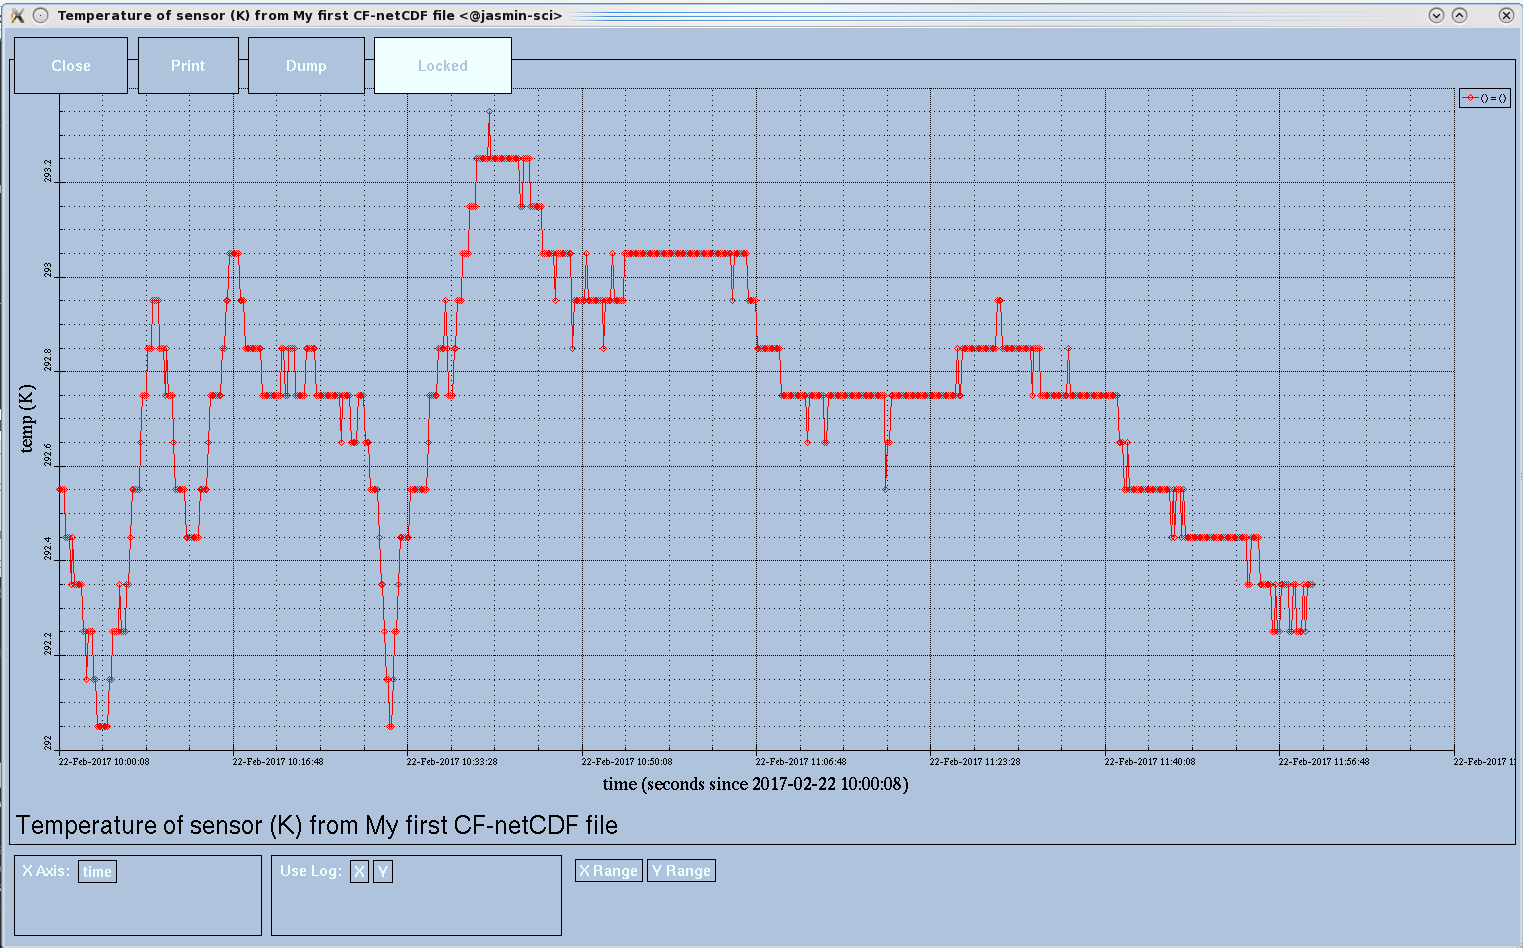
\includegraphics[width=0.7\textwidth]{sensor-data-ncview.png}

Obviously, this is not publication quality!

\end{frame}
\begin{frame}[fragile]
    \frametitle{Plotting data with \texttt{matplotlib}}

\begin{minted}[bgcolor=lightyellow]{python}
#!/usr/bin/env python

''' Plots a line graph from a NetCDF file '''

from netCDF4 import Dataset
import numpy as np

datafile = 'sensor_data.nc'

nc = Dataset(datafile, mode='r')

temps = nc.variables['temp'][:]
times = nc.variables['time'][:]

times = num2date(time[:],units=time.units, calendar=time.calendar)

plt.plot_date(times,temps)
plt.savefig('sensor_data.png')
\end{minted}

\end{frame}
\begin{frame}[fragile]
\frametitle{Plotting data - with labels}

After
\texttt{times = num2date(time\{:\},units=time.units, calendar=time.calendar)}

\begin{minted}[bgcolor=lightyellow]{python}
#get "handles" to affect plot styling
fig, ax = plt.subplots()
#tick every tenth minute
ax.xaxis.set_major_locator(MinuteLocator(byminute=range(0,60,10)))

#format of date on x-axis (display minutes, uses strftime)
ax.xaxis.set_major_formatter(DateFormatter('%H:%M'))

#tick every minute
ax.xaxis.set_minor_locator(MinuteLocator())
ax.autoscale_view()

#line graph
plt.plot_date(times,temps,'-')
labels = ax.get_xticklabels()
plt.setp(labels, rotation=90, fontsize=10, horizontalalignment='center')
plt.xlabel(time.standard_name)
plt.ylabel(temp.standard_name + ' / ' + temp.units)
plt.title(nc.title)

#tidy up layout automatically
fig.tight_layout()

plt.savefig('sensor_data.png')
\end{minted}

(see \texttt{python/exercises/example\_code/plot-netcdf.py} in your
\texttt{git} checkout)

\end{frame}
\begin{frame}[fragile]
\frametitle{Plotting data with CIS (Community Intercomparison
Suite)}

Another option is CIS

\emph{``CIS is an open source command-line tool for easy collocation,
visualization, analysis, and comparison of diverse gridded and ungridded
datasets used in the atmospheric sciences''}

It is based on python. Homepage:
\url{http://www.cistools.net/}

\begin{verbatim}
cis plot temp:sensor_data.nc --xaxis time --yaxis temp \ 
    --title "Papouch Thermometer Data, 2017-02-22, UoL PRD" --xstep "0.010416"  \ 
    --output sensor_data_sample.svg
\end{verbatim}
\end{frame}
\begin{frame}

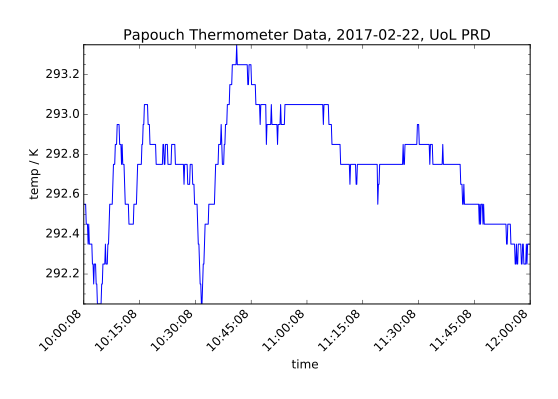
\includegraphics[width=\textwidth]{sensor_data_sample}

\end{frame}
\begin{frame}
\frametitle{Further exercises}

\begin{block}{Command-line options}

e.g. using \texttt{optparse} (for Python \textless{} v2.7) or
\texttt{argparse} (Python ≥ 2.7)
\end{block}
\end{frame}
\end{document}
